\documentclass[pdftex,12pt,a4paper]{article}

\usepackage{graphicx}  
\usepackage[margin=2.5cm]{geometry}
\usepackage{breakcites}
\usepackage{indentfirst}
\usepackage{pgfgantt}
\usepackage{pdflscape}
\usepackage{float}
\usepackage{epsfig}
\usepackage{epstopdf}
\usepackage[cmex10]{amsmath}
\usepackage{stfloats}
\usepackage{multirow}
\usepackage{karnaugh-map}
\usepackage{amssymb}
\usepackage{amsbsy}
\usepackage{placeins}


\renewcommand{\refname}{REFERENCES}
\linespread{1.3}

\usepackage{mathtools}
%\newcommand{\HRule}{\rule{\linewidth}{0.5mm}}
\thispagestyle{empty}
\begin{document}
\begin{titlepage}
\begin{center}
\textbf{}\\
\textbf{\Large{ISTANBUL TECHNICAL UNIVERSITY}}\\
\vspace{0.5cm}
\textbf{\Large{COMPUTER ENGINEERING DEPARTMENT}}\\
\vspace{2cm}
\textbf{\Large{BLG 242E\\ DIGITAL CIRCUITS LABORATORY\\ EXPERIMENT REPORT}}\\
\vspace{2.8cm}
\begin{table}[ht]
\centering
\Large{
\begin{tabular}{lcl}
\textbf{EXPERIMENT NO}  & : & 3 \\
\textbf{EXPERIMENT DATE}  & : & 28.02.2020 \\
\textbf{LAB SESSION}  & : & FRIDAY - 08.30 \\
\textbf{GROUP NO}  & : & G6 \\
\end{tabular}}
\end{table}
\vspace{1cm}
\textbf{\Large{GROUP MEMBERS:}}\\
\begin{table}[ht]
\centering
\Large{
\begin{tabular}{rcl}
150170087  & : & Sırrı Batuhan ÇOKSAK \\
150170039  & : & Fatih MURAT \\
150180905  & : & Fatima RAHİMOVA(G9) \\
\end{tabular}}
\end{table}
\vspace{2.8cm}
\textbf{\Large{SPRING 2020}}

\end{center}

\end{titlepage}

\thispagestyle{empty}
\addtocontents{toc}{\contentsline {section}{\numberline {}FRONT COVER}{}}
\addtocontents{toc}{\contentsline {section}{\numberline {}ETHICS}{}}
\addtocontents{toc}{\contentsline {section}{\numberline {}CONTENTS}{}}
\setcounter{tocdepth}{4}
\tableofcontents
\clearpage

\setcounter{page}{1}

\section{INTRODUCTION}

In this experiment, we were expected to find the prime implicants and the implementations of them with the lowest cost of the given function. We experienced well-known methods such as karnaugh map and Quine-McCluskey algorithm. Beside that, we converted given expressions each other with the given constrains. While doing these, we used AND, OR, NOT, NAND gates, multiplexers and decoders.

\section{MATERIALS AND EXPERIMENT}
\underline{Tools Used}
\begin{itemize}
    \item C.A.D.E.T
    \item 74000 series ICs
    \begin{itemize}
        \item 74xx00 - Quadruple 2-input Positive NAND Gates
        \item 74xx04 - Hex Inverters     
        \item 74xx08 - Quadruple 2-input Positive AND Gates
        \item 74xx10 - Triple 3-input Positive NAND Gates
        \item 74xx11 - Triple 3-input Positive AND Gates
        \item 74xx32 - Quadruple 2-input Positive OR Gates
        \item 74xx138 - 3:8 Decoder
        \item 74xx151 - 8:1 Multiplexer
    \end{itemize}
\end{itemize}
\clearpage
\subsection{PART 1}
\paragraph{}
In the first part of the experiment, we were given set of 1-generators and set of don't cares of the function $F_{1}$. From this information, we drew the karnaugh map easily and selected the all prime implicants. For all prime implicants we had cost values(2 for each variable and 1 for complement operation).


\begin{itemize}
    \item $F_{1}$(a,b,c,d) = $U_{1}$(0, 3, 5, 7, 11, 12, 13) + $U_{\Phi}$(1, 8, 15)  
\end{itemize}

\begin{figure}[!h]
\begin{karnaugh-map}[4][4][1][$c d$][$a b$]
\minterms{0,3,5,7,11,12,13}
\terms{1,8,15}{${\Phi}$}
\terms{2,4,6,9,10,14}{0}
\implicant{0}{1}
\implicant{3}{11}
\implicant{12}{8}
\implicant{5}{15}
\implicant{1}{7}
\implicant{12}{13}
\implicantedge{0}{0}{8}{8}

\end{karnaugh-map}
\centering
\caption{Karnaugh map of $F$}
\label{karnaugh1}
\end{figure}


\begin{table}[h]
\begin{tabular}{cccccccc}
              & $a'b'c'$  &  $b'c'd'$   &   $a'd$    &   $cd$   &   $bd$    &      $abc'$   &   $ac'd'$ \\
SYMBOL         & A            & B            & C           & D      & E             & F           & G          \\
COVERED POINTS & 0,1       & 0,8     &    1,3,5,7   &    3,7,11,15  & 5,7,13,15     & 12,13       & 8, 12       \\
COST           & 9            & 9            & 5           & 4      & 4             & 7           & 8        \\
\end{tabular}

\caption{All prime implicants}
\label{ponisandta}
\end{table}

\clearpage


\paragraph{}
In order to choose proper prime implicants with the lowest cost, we used prime implicant chart method. We did not include the don't care values to our prime implicant chart since we did not need them anymore. Since D is the distinguished point for 11, we had to choose it. After we chose D, we eliminated the D as a row and other covering columns(3,7,11).
\newline
\newline
\begin{table}[h]
\centering
\begin{tabular}{l|l|l|l|l|l|l|l|l|}
\cline{2-9}
                        & 0 & 3 & 5 & 7 & 11                        & 12 & 13 & COST \\ \hline
\multicolumn{1}{|l|}{A} & x &   &   &   &                           &    &    & 9    \\ \hline
\multicolumn{1}{|l|}{B} & x &   &   &   &                           &    &    & 9    \\ \hline
\multicolumn{1}{|l|}{C} &   & x & x & x &                           &    &    & 5    \\ \hline
\multicolumn{1}{|l|}{D} &   & x &   & x & {\color[HTML]{FE0000} x}  &    &    & 4    \\ \hline
\multicolumn{1}{|l|}{E} &   &   & x & x &                           &    & x  & 4    \\ \hline
\multicolumn{1}{|l|}{F} &   &   &   &   &                           & x  & x  & 7   \\ \hline
\multicolumn{1}{|l|}{G} &   &   &   &   &                           & x  &    & 8   \\ \hline
\end{tabular}
\caption{Prime implicant chart.}
\label{primeimplicantchart1}
\end{table}

\paragraph{}
After the first elimination operation we had new chart(Table 3). In this chart, we had no distinguished points, therefore we compared them each other to pick proper prime implicant with lower cost. Since A and B are the exactly same prime implicant in terms of coverage and cost, we were able to pick one of them. For this experiment, we chose A. After that, we eliminate the A and B's row and related column(0).
\newline
\newline


\begin{table}[h]
\centering
\begin{tabular}{l|l|l|l|l|l|}
\cline{2-6}
                        & 0 & 5 &  12 & 13 & COST \\ \hline
\multicolumn{1}{|l|}{A} & x &   &     &    & 9    \\ \hline
\multicolumn{1}{|l|}{B} & x &   &     &    & 9    \\ \hline
\multicolumn{1}{|l|}{C} &   & x &     &    & 5    \\ \hline
\multicolumn{1}{|l|}{E} &   & x &     & x  & 4    \\ \hline
\multicolumn{1}{|l|}{F} &   &   &  x  & x  & 7   \\ \hline
\multicolumn{1}{|l|}{G} &   &   &  x  &    & 8   \\ \hline
\end{tabular}
\caption{Prime implicant chart after first elimination.}
\label{primeimplicantchart2}
\end{table}

\clearpage

\paragraph{}
After the second elimination operation, we had another new chart(Table 4). In this step, we compared C and E. As it is obvious that E covers C with lower cost, we chose E. After we chose E, we eliminated related rows(C,E) and columns(5,13).
\newline
\newline



\begin{table}[h]
\centering
\begin{tabular}{l|l|l|l|l|}
\cline{2-5}
                        & 5 &  12 & 13 & COST \\ \hline
\multicolumn{1}{|l|}{C} & x &     &    & 5    \\ \hline
\multicolumn{1}{|l|}{E} & x &     & x  & 4    \\ \hline
\multicolumn{1}{|l|}{F} &   &  x  & x  & 7   \\ \hline
\multicolumn{1}{|l|}{G} &   &  x  &    & 8   \\ \hline
\end{tabular}
\caption{Prime implicant chart after second elimination.}
\label{primeimplicantchart3}
\end{table}

\paragraph{}
After the last elimination operation, we were left with F and G for the same point(12). Since F has lower cost than G, we chose F as our last prime implicant. After the elimination, nothing left and we are done with elimination part.
\newline
\newline

\begin{table}[h]
\centering
\begin{tabular}{l|l|l|}
\cline{2-3}
                         &  12 & COST \\ \hline
\multicolumn{1}{|l|}{F}  &  x  & 7   \\ \hline
\multicolumn{1}{|l|}{G}  &  x  & 8   \\ \hline
\end{tabular}
\caption{Prime implicant chart after third elimination.}
\label{primeimplicantchart4}
\end{table}

\clearpage

\paragraph{}
As a result of these eliminations, we chose A, D, E and F with 24 total cost. Chosen prime implicants is shown on karnaugh map in Figure 2.

\begin{figure}[!h]
\begin{karnaugh-map}[4][4][1][$c d$][$a b$]
\minterms{0,3,5,7,11,12,13}
\terms{1,8,15}{${\Phi}$}
\terms{2,4,6,9,10,14}{0}
\implicant{0}{1}
\implicant{3}{11}
\implicant{5}{15}
\implicant{12}{13}

\end{karnaugh-map}
\centering
\caption{Karnaugh map of $F$}
\label{karnaugh2}
\end{figure}

\paragraph{}
After the karnaugh map elimination operations, we were supposed to use Quine-McCluskey method. Algorithm steps are shown one by one below. Results from Quine-McCluskey method and karnaugh map verified each other and gave exact same prime implicants as it was expected.
\newline


\begin{table}[h]
\centering
\begin{tabular}{c|c|c}
Number  & a b c d &             \\ \hline
0       & 0 0 0 0 & \checkmark \\ \hline 
1       & 0 0 0 1 &  \checkmark\\ 
8       & 1 0 0 0 &  \checkmark\\ \hline
3       & 0 0 1 1 &  \checkmark\\ 
5       & 0 1 0 1 &  \checkmark\\ 
12      & 1 1 0 0 &  \checkmark\\ \hline
7       & 0 1 1 1 &  \checkmark\\ 
11      & 1 0 1 1 &  \checkmark\\
13      & 1 1 0 1 &  \checkmark\\ \hline
15      & 1 1 1 1 &  \checkmark\\ 
\end{tabular}
\caption{Quine-McCluskey algorithm step-1}
\label{quine1}
\end{table}
\clearpage
\begin{table}[h]
\centering
\begin{tabular}{c|c|c}
Number  & a b c d &              \\ \hline
0,1     & 0 0 0 - &  Prime I.(a'b'c')            \\ 
0,8     & - 0 0 1 &  Prime I.(b'c'd)            \\ \hline
1,3     & 0 0 - 1 &\checkmark  \\ 
1,5     & 0 - 0 1 & \checkmark \\ 
8,12    & 1 - 0 0 &  Prime I.(ac'd')            \\ \hline
3,7     & 0 - 1 1 & \checkmark \\ 
3,11    & - 0 1 1 & \checkmark \\ 
5,7     & 0 1 - 1 & \checkmark \\
12,13   & 1 1 0 - &  Prime I.(abc')            \\ \hline
7,15    & - 1 1 1 & \checkmark \\ 
11,15   & 1 - 1 1 & \checkmark \\
13,15   & 1 1 - 1 & \checkmark \\
\end{tabular}
\caption{Quine-McCluskey algorithm step-2}
\label{quine2}
\end{table}

\paragraph{}
As it is been seen in the Table 8, there exists same expressions more than one. However, we use only one of the same ones.

\begin{table}[h]
\centering
\begin{tabular}{c|c|c}
Number  & a b c d &      \\ \hline
1,3,5,7     & 0 - - 1 & Prime I.(a'd)   \\ 
1,5,3,7     & 0 - - 1 & Prime I.(a'd)    \\ \hline
3,7,11,15   & - - 1 1 & Prime I.(cd) \\ 
3,11,7,15   & - - 1 1 & Prime I.(cd) \\ 
5,7,13,15   & - 1 - 1 & Prime I.(bd)   \\ 
\end{tabular}
\caption{Quine-McCluskey algorithm step-3}
\label{quine3}
\end{table}
\clearpage

\paragraph{}
As a result of all of these operations, we determined our F function and its truth table as shown below;
\begin{itemize}
    \item  F(a,b,c,d) = a'b'c' + cd + bd + abc'
\end{itemize}


\begin{table}[h]
\centering
\begin{tabular}{|c|c|c|c|c|c|c|c|c|c|c|c|}
\hline
a & b & c & d & a' & b' & c' & a'b'c' & cd & bd & abc' & F(a,b,c,d) \\ \hline
0 & 0 & 0 & 0 & 1  & 1  & 1  & 1      & 0  & 0  & 0    & 1          \\ 
0 & 0 & 0 & 1 & 1  & 1  & 1  & 1      & 0  & 0  & 0    & ${\Phi}$          \\ 
0 & 0 & 1 & 0 & 1  & 1  & 0  & 0      & 0  & 0  & 0    & 0          \\ 
0 & 0 & 1 & 1 & 1  & 1  & 0  & 0      & 1  & 0  & 0    & 1          \\ 
0 & 1 & 0 & 0 & 1  & 0  & 1  & 0      & 0  & 0  & 0    & 0          \\ 
0 & 1 & 0 & 1 & 1  & 0  & 1  & 0      & 0  & 1  & 0    & 1          \\
0 & 1 & 1 & 0 & 1  & 0  & 0  & 0      & 0  & 0  & 0    & 0          \\ 
0 & 1 & 1 & 1 & 1  & 0  & 0  & 0      & 1  & 1  & 0    & 1          \\ 
1 & 0 & 0 & 0 & 0  & 1  & 1  & 0      & 0  & 0  & 0    & ${\Phi}$          \\ 
1 & 0 & 0 & 1 & 0  & 1  & 1  & 0      & 0  & 0  & 0    & 0          \\ 
1 & 0 & 1 & 0 & 0  & 1  & 0  & 0      & 0  & 0  & 0    & 0          \\ 
1 & 0 & 1 & 1 & 0  & 1  & 0  & 0      & 1  & 0  & 0    & 1          \\ 
1 & 1 & 0 & 0 & 0  & 0  & 1  & 0      & 0  & 0  & 1    & 1          \\ 
1 & 1 & 0 & 1 & 0  & 0  & 1  & 0      & 0  & 1  & 1    & 1          \\
1 & 1 & 1 & 0 & 0  & 0  & 0  & 0      & 0  & 0  & 0    & 0          \\ 
1 & 1 & 1 & 1 & 0  & 0  & 0  & 0      & 1  & 1  & 0    & ${\Phi}$          \\ \hline
\end{tabular}
\caption{Truth table for F(a,b,c,d)}
\label{truth1}
\end{table}

\clearpage


\paragraph{}
We implemented our expression using AND, OR and NOT gates as shown below;

\begin{figure}[!h]
	\centering
	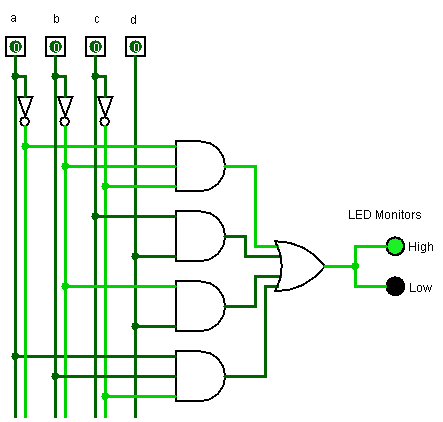
\includegraphics[width=0.5\textwidth]{part1.png}	
	\caption{Circuit of $F(a,b,c,d)$}
	\label{log1}
\end{figure}

\clearpage

\subsection{PART 2}

\paragraph{}
In the second part of the experiment, we were expected to express our F function that we obtained from part-1 by using only NAND and NOT gates and implement the proper circuit.

\begin{itemize}
    \item  F(a,b,c,d) = a'b'c' + cd + bd + abc' (AND, OR, NOT gates are used)
    \item F(a,b,c,d) = (([(a'b'c')'(cd)'(bd)']')'(abc')')' (NAND and NOT gates are used)
\end{itemize}

\paragraph{}
Implementation of the F function using by only NAND and NOT gates is as shown in Figure 4;

\begin{figure}[!h]
	\centering
	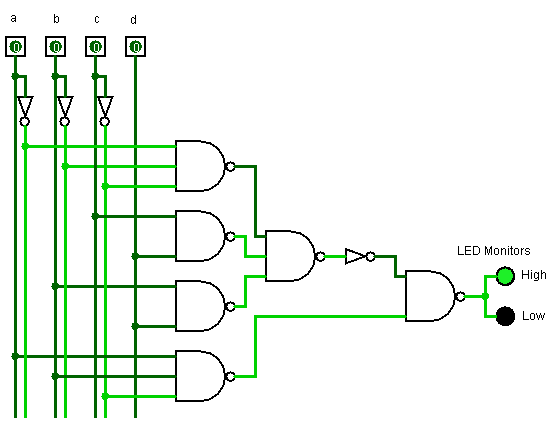
\includegraphics[width=0.7\textwidth]{part2.png}	
	\caption{Circuit of $F(a,b,c,d)$}
	\label{log2}
\end{figure}

\paragraph{}
As these 2 expression is same in terms of outputs values, truth tables of them are also same.
\clearpage
\subsection{PART 3}

\paragraph{}
In the third part of the experiment, we were expected design and draw the same function using a single 8:1 multiplexer and NOT gates. In order to do that, we chose a,b and c input variables as selector input and d as input. Beside that, we assumed that enable input is always 1 and we did not show that in the logisim implementation. However, during the experiment we used ICs that requires enable input which we connected to high voltage. In this context, we obtained out truth table and the circuit implementation as shown below;
\newline
\newline

\begin{figure}[!h]
	\centering
	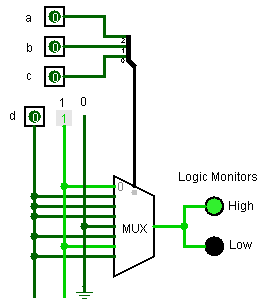
\includegraphics[width=0.55\textwidth]{part3.png}	
	\caption{Circuit of $F(a,b,c,d)$}
	\label{log3}
\end{figure}


\clearpage

\begin{table}
\centering
    \begin{tabular}{|c|c|c|c|c|c|c|}
    \hline
         A & B & C & D & F &     \\ \hline
         0 & 0 & 0 & 0 & 1 & \multirow{2}{1em}{1} \\
         0 & 0 & 0 & 1 & ${\Phi}$ & \\\hline
         0 & 0 & 1 & 0 & 0 & \multirow{2}{1em}{d}\\
         0 & 0 & 1 & 1 & 1 & \\\hline
         0 & 1 & 0 & 0 & 0 & \multirow{2}{1em}{d}\\
         0 & 1 & 0 & 1 & 1 & \\\hline
         0 & 1 & 1 & 0 & 0 & \multirow{2}{1em}{d}\\
         0 & 1 & 1 & 1 & 1 & \\\hline
         1 & 0 & 0 & 0 & ${\Phi}$ & \multirow{2}{1em}{0} \\
         1 & 0 & 0 & 1 & 0 & \\\hline
         1 & 0 & 1 & 0 & 0 & \multirow{2}{1em}{d}\\
         1 & 0 & 1 & 1 & 1 & \\\hline
         1 & 1 & 0 & 0 & 1 & \multirow{2}{1em}{1}\\
         1 & 1 & 0 & 1 & 1 & \\\hline
         1 & 1 & 1 & 0 & 0 & \multirow{2}{1em}{0}\\
         1 & 1 & 1 & 1 & ${\Phi}$ & \\
         \hline
    \end{tabular}
    \caption{Truth table for multiplexer implementation.}
    \label{truth2}
\end{table}


\clearpage
\subsection{PART 4}

\paragraph{}
In the fourth and last part of the experiment, we were expected to design and draw the functions below using a single 3:8 decoder, OR, and NOT gates.

\begin{itemize}
    \item $F_{1}$(a, b, c) = a'c' + bc
    \item $F_{2}$(a, b, c) = a'b'c' + ab
\end{itemize}

For the $F_{1}$ we drew the truth table and after that, we implemented our function as expected. But there was a important point in the lab session for this implementation; decoder was outputting the inverted form of the expressions. Therefore we needed to implement extra inverters to obtain normal forms(not inverted version) of the outputs. With this touch, we got the expected and correct outputs from the logic monitors.\newline
\begin{table}[h]
\centering
\begin{tabular}{|c|c|c|c|c|c|c|c|c|}
\hline
a & b & c & a' & b' & c' & $a' \cdot c'$ & $b \cdot c$ & $F_{1}$ = $a' \cdot c'$ + $b \cdot c$     \\ \hline
0 & 0 & 0 & 1  & 1  & 1  & 1             & 0      & 1             \\ \hline
0 & 0 & 1 & 1  & 1  & 0  & 0             & 0      & 0               \\ \hline
0 & 1 & 0 & 1  & 0  & 1  & 1             & 0      & 1              \\ \hline
0 & 1 & 1 & 1  & 0  & 0  & 0             & 1      & 1               \\ \hline
1 & 0 & 0 & 0  & 1  & 1  & 0             & 0      & 0               \\ \hline
1 & 0 & 1 & 0  & 1  & 0  & 0             & 0      & 0           \\ \hline
1 & 1 & 0 & 0  & 0  & 1  & 0             & 0      & 0          \\ \hline
1 & 1 & 1 & 0  & 0  & 0  & 0             & 1      & 1               \\ \hline
\end{tabular}
\caption{Truth table for $F_{1}$}
\label{truth3}
\end{table}

\paragraph{}
After we drew truth table for $F_{1}$, we implemented our circuit in this way;

\begin{figure}[!h]
	\centering
	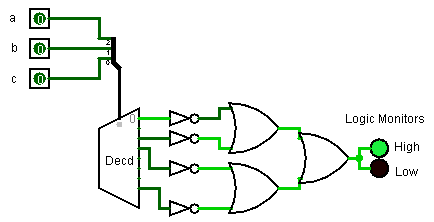
\includegraphics[width=0.55\textwidth]{part4-1.png}	
	\caption{Circuit of $F_{1}(a,b,c,d)$}
	\label{log4}
\end{figure}
\clearpage

\paragraph{}
For the $F_{2}$ we did the same operations as we did for $F_{1}$. Simply, we drew the truth table and implemented our circuit as the truth table verified our implementation. Decoder was giving inverted version of the output values as well. Therefore we used inverters to control this situtation again. As we assumed that enable input is always 1 for the former implementations, we did it for the $F_{2}$ implementation as well. As a result we obtained both truth table and circuit design as below;\newline

\begin{table}[!h]
\centering
\begin{tabular}{|c|c|c|c|c|c|c|c|c|}
\hline
a & b & c & a' & b' & c' & $a' \cdot b' \cdot c'$ & $a \cdot b$ & $F_{2}$ = $a' \cdot b' \cdot c'$ + $a \cdot b$      \\ \hline
0 & 0 & 0 & 1  & 1  & 1  & 1             & 0      & 1             \\ \hline
0 & 0 & 1 & 1  & 1  & 0  & 0             & 0      & 0               \\ \hline
0 & 1 & 0 & 1  & 0  & 1  & 0             & 0      & 0              \\ \hline
0 & 1 & 1 & 1  & 0  & 0  & 0             & 0      & 0               \\ \hline
1 & 0 & 0 & 0  & 1  & 1  & 0             & 0      & 0               \\ \hline
1 & 0 & 1 & 0  & 1  & 0  & 0             & 0      & 0           \\ \hline
1 & 1 & 0 & 0  & 0  & 1  & 0             & 1      & 1          \\ \hline
1 & 1 & 1 & 0  & 0  & 0  & 0             & 1      & 1               \\ \hline
\end{tabular}
\caption{Truth table for $F_{2}$}
\label{truth4}
\end{table}

\begin{figure}[!h]
	\centering
	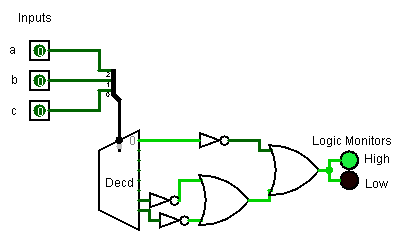
\includegraphics[width=0.55\textwidth]{part4-2.png}	
	\caption{Circuit of $F_{2}(a,b,c,d)$}
	\label{log5}
\end{figure}

\clearpage
\section{RESULTS}
Throughout the whole experiment the results we obtained was not different from the expected results which we calculated before the implementation of the functions and expressions. Since the equipment we used during the experiment were mostly integrated circuits results were output values of these equipment and the results was certain either one or zero. Hence, we obtained precise results and verified our results using truth tables.


\section{DISCUSSION}
Generally, the results we found were the same with  theoretically as they should have been. In the first part of the experiment, we couldn't get a result for a long time because we plugged the IC in reverse, which caused us to lose time. Other than that, we had some difficulties in the part 3 of the experiment . We could not figure out the pin configuration of 74151 - 8-Input Multiplexer but with the help of the laboratory assistant, we solved the problem and achieved the result. Except for this problem we did not face big problems and outputs of the each part of the experiment in logic monitor met the result we expected.

\section{CONCLUSION}
As a result, the experiment wasn't too hard but as we mentioned in the discussion part since we did not notice that we had the IC upside down for a long time, there was not enough time left to do $F_{2}$ in the fourth part of this experiment. But all in all, we have successfully completed the experiment without harming any IC, cabel etc. in the Logic Circuits Laboratory. Moreover, thanks to this session, we especially concreted our multiplexer and decoder knowledge and practical skills.


\newpage
\addcontentsline{toc}{section}{\numberline {}REFERENCES}
[1] Istanbul Technical University Department of Computer Engineering BLG-242E Logic Circuits Laboratory Experiments Booklet Version 1.9.1, spring 2020.
\newline
[2] Overleaf documentation https://tr.overleaf.com/learn.

\bibliographystyle{unsrt}
\bibliography{reference}

\end{document}

